\chapter{Complexation}\label{ch:b1:complexation}

Versons un peu de solution d'ammoniac dans du sulfate de cuivre(II) bleu
pâle~: un précipité bleu pâle se forme aussitôt. Versons-en davantage,
et le précipité se dissout en une solution d'un bleu profond, presque
celui de l'encre. Rien, dans les chapitres sur les acides et les bases ou
sur la précipitation, n'explique cette seconde étape. Les molécules
d'ammoniac se sont liées à l'ion cuivre par leurs \omterm{def:b1:lewis-resonance-vsepr:lewis}{doublets non liants} et
ont formé une espèce nouvelle, un \omterm{def:b1:complexation:complex}{complexe}, plus stable que l'hydroxyde
et d'une autre couleur. Les \omterm{def:b1:complexation:complex}{complexes} transportent l'oxygène dans le
sang, retiennent le métal de la chlorophylle et de la vitamine B$_{12}$,
adoucissent les eaux dures et dissolvent des métaux que rien d'autre
n'attaque. Ce chapitre les traite comme un échange de particules de plus
dans l'eau, avec ses propres constantes et ses propres diagrammes.

\begin{recall}
Les \omterm{def:b1:lewis-resonance-vsepr:lewis-acid}{acides de Lewis} (accepteurs de doublets), les \omterm{def:b1:lewis-resonance-vsepr:lewis-acid}{bases de Lewis}
(donneurs de doublets) et la \omterm{def:b1:lewis-resonance-vsepr:lewis-acid}{liaison dative} ont été définis au
\cref{ch:b1:lewis-resonance-vsepr}. Les \omterm{def:b1:predominant-reaction:predominance}{diagrammes de prédominance} et la
méthode de la \omterm{def:b1:predominant-reaction:predominant-reaction}{réaction prépondérante} viennent du
\cref{ch:b1:predominant-reaction}~; le \omterm{def:b1:precipitation:solubility-product}{produit de solubilité} et la
condition de précipitation, du \cref{ch:b1:precipitation}.
\end{recall}

\begin{omfigure}
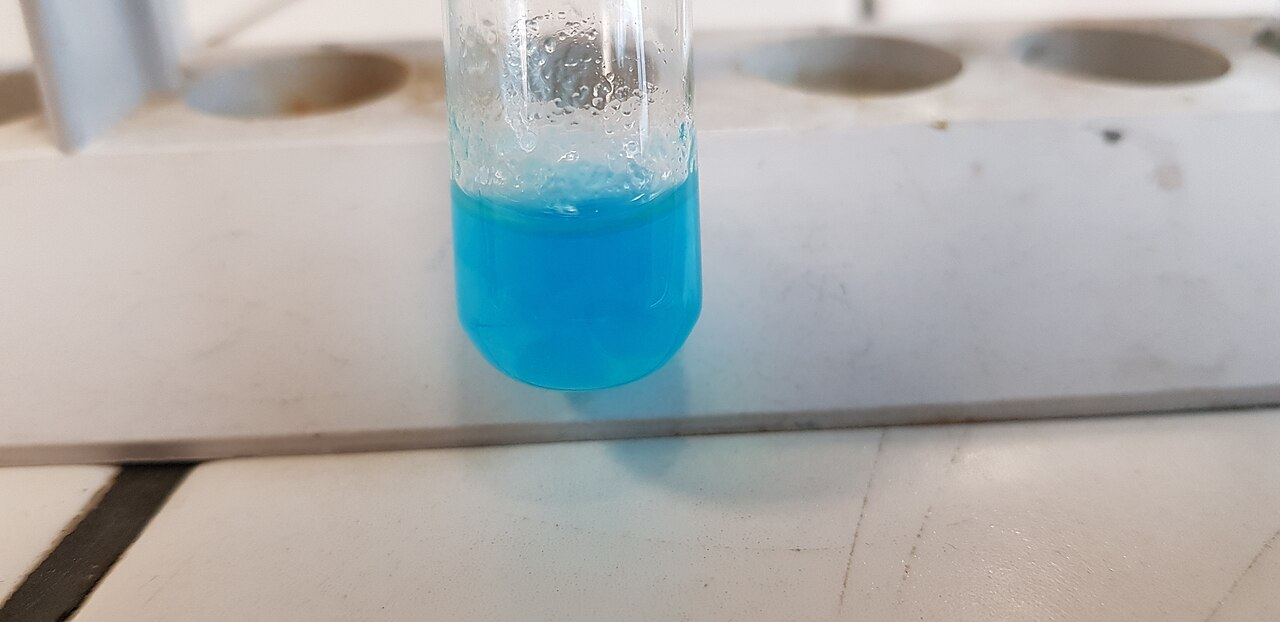
\includegraphics[height=4.2cm]{images/book2/copper-hydroxide.jpg}\hspace{0.6em}%
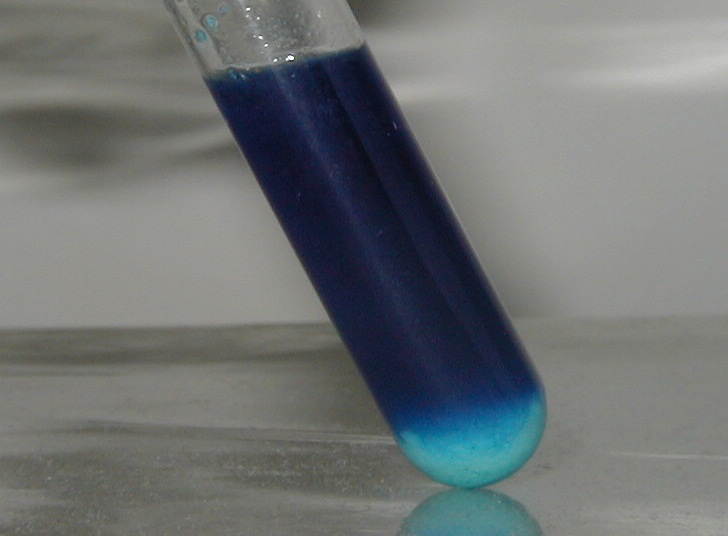
\includegraphics[height=4.2cm]{images/book2/copper-ammine.jpg}

{\small À gauche~: une suspension d'hydroxyde de cuivre(II) bleu pâle
(photographie Alvy16, CC BY 4.0). À droite~: avec plus d'ammoniac, le
solide se dissout en donnant l'ion tétraamminecuivre(II), bleu profond~;
un peu d'hydroxyde non dissous reste au fond du tube (photographie
Chemicalinterest, domaine public). Toutes deux sur Wikimedia Commons.}
\end{omfigure}

\section{Complexes et ligands}

\begin{definition}[Complexe, atome central, ligand]\label{def:b1:complexation:complex}
Un \emph{complexe}\index{complexe} est une espèce formée d'un \emph{atome
central}\index{atome central} ou d'un ion central, en général un cation
métallique jouant le rôle d'\omterm{def:b1:lewis-resonance-vsepr:lewis-acid}{acide de Lewis}, lié par des \omterm{def:b1:lewis-resonance-vsepr:lewis-acid}{liaisons datives}
à des molécules ou à des ions jouant le rôle de \omterm{def:b1:lewis-resonance-vsepr:lewis-acid}{bases de Lewis}, les
\emph{ligands}\index{ligand}. Sa formule s'écrit entre crochets, avec sa
charge totale~: $[\ce{Cu(NH3)4}]^{2+}$,
$[\ce{Fe(CN)6}]^{4-}$, $[\ce{Ag(NH3)2}]^{+}$, $[\ce{FeSCN}]^{2+}$.
\end{definition}

La charge du \omterm{def:b1:complexation:complex}{complexe} est la somme des charges de l'ion central et des
\omterm{def:b1:complexation:complex}{ligands}~: $\mathrm{Fe^{2+}}$ et six \ce{CN-} donnent
$[\ce{Fe(CN)6}]^{4-}$. Un \omterm{def:b1:complexation:complex}{ligand} doit posséder au moins un \omterm{def:b1:lewis-resonance-vsepr:lewis}{doublet non
liant}~: \ce{NH3}, \ce{H2O}, \ce{OH-}, \ce{Cl-}, \ce{CN-}, \ce{SCN-} (lié
par S ou par N). Tout ion métallique dans l'eau est en fait déjà un
\omterm{def:b1:complexation:complex}{complexe} dont les \omterm{def:b1:complexation:complex}{ligands} sont des molécules d'eau,
$[\ce{Cu(H2O)6}]^{2+}$ ou $[\ce{Fe(H2O)6}]^{3+}$~; former un autre
\omterm{def:b1:complexation:complex}{complexe} revient à échanger ces molécules d'eau contre d'autres \omterm{def:b1:complexation:complex}{ligands},
et l'on omet les \omterm{def:b1:complexation:complex}{ligands} aqua dans les formules, comme on écrit \ce{H3O+}
pour le proton hydraté.

\begin{omfigure}
\begin{tikzpicture}[font=\small, line cap=round]
  % [Ag(NH3)2]+ : linear
  \begin{scope}
    \node (ag) at (0,0) {\ce{Ag}};
    \node (n1) at (-1.2,0) {\ce{H3N}};
    \node (n2) at (1.2,0) {\ce{NH3}};
    \draw[thick] (n1) -- (ag) -- (n2);
    \node at (0,-1.75) {$[\ce{Ag(NH3)2}]^{+}$, linéaire};
  \end{scope}
  % [Cu(NH3)4]2+ : square plane in perspective
  \begin{scope}[xshift=4.3cm, every node/.style={fill=white, inner sep=1.5pt}]
    \node (cu) at (0,0) {\ce{Cu}};
    \node (a) at (-1.45,-0.5) {\ce{H3N}};
    \node (b) at (1.45,0.5) {\ce{NH3}};
    \node (c) at (0.85,-0.9) {\ce{NH3}};
    \node (d) at (-0.85,0.9) {\ce{H3N}};
    \begin{pgfonlayer}{background}
    \draw[gray, dashed] (a.center) -- (c.center) -- (b.center) -- (d.center) -- cycle;
    \end{pgfonlayer}
    \draw[thick] (cu) -- (a); \draw[thick] (cu) -- (b);
    \draw[thick] (cu) -- (c); \draw[thick] (cu) -- (d);
    \node at (0,-1.75) {$[\ce{Cu(NH3)4}]^{2+}$, plan carré};
  \end{scope}
  % [Fe(CN)6]4- : octahedron
  \begin{scope}[xshift=9.2cm, every node/.style={fill=white, inner sep=1.5pt}]
    \node (fe) at (0,0) {\ce{Fe}};
    \node (t) at (0,1.3) {\ce{CN}};
    \node (u) at (0,-1.3) {\ce{CN}};
    \node (l) at (-1.45,-0.45) {\ce{NC}};
    \node (r) at (1.45,0.45) {\ce{CN}};
    \node (f) at (0.8,-0.8) {\ce{CN}};
    \node (k) at (-0.8,0.8) {\ce{NC}};
    \begin{pgfonlayer}{background}
    \draw[gray, dashed] (l.center) -- (f.center) -- (r.center) -- (k.center) -- cycle;
    \end{pgfonlayer}
    \foreach \x in {t,u,l,r,f,k} \draw[thick] (fe) -- (\x);
    \node at (0,-1.75) {$[\ce{Fe(CN)6}]^{4-}$, octaédrique};
  \end{scope}
\end{tikzpicture}

{\small Trois \omterm{def:b1:complexation:complex}{complexes} et leurs géométries. Chaque trait est une \omterm{def:b1:lewis-resonance-vsepr:lewis-acid}{liaison
dative} allant du \omterm{def:b1:lewis-resonance-vsepr:lewis}{doublet non liant} du \omterm{def:b1:complexation:complex}{ligand} (le N de l'ammoniac, le C
du cyanure) vers l'ion métallique~; les tirets dessinent le carré de
quatre \omterm{def:b1:complexation:complex}{ligands}. La géométrie des \omterm{def:b1:complexation:complex}{complexes} est expliquée dans le volume
de deuxième année.}
\end{omfigure}

\begin{definition}[Ligand polydenté, chélate]\label{def:b1:complexation:chelate}
Un \omterm{def:b1:complexation:complex}{ligand} qui se lie au même ion central par plusieurs de ses atomes à
la fois est un \emph{ligand polydenté}\index{ligand polydente@ligand polydenté}~; le \omterm{def:b1:complexation:complex}{complexe}
qu'il forme, dans lequel le \omterm{def:b1:complexation:complex}{ligand} ferme des cycles autour de l'ion
métallique, est un \emph{chélate}\index{chelate@chélate}. L'éthylènediamine
\ce{H2N-CH2-CH2-NH2} se lie par deux atomes N, l'ion oxalate
\ce{C2O4^2-} par deux atomes O, et l'ion éthylènediaminetétraacétate
(\emph{edta}, noté \ce{Y^4-}) par deux atomes N et quatre atomes O.
\end{definition}

\begin{omfigure}
\setchemfig{atom sep=1.9em}
\chemfig{N(-[3]-[2]C(=[1]O)-[3]O^{-})(-[5]-[6]C(=[7]O)-[5]O^{-})-[0]-[0]N(-[1]-[2]C(=[3]O)-[1]O^{-})(-[7]-[6]C(=[5]O)-[7]O^{-})}
\hspace{2.2em}
\begin{tikzpicture}[font=\small, baseline=(ca.base)]
  \node[circle, draw, thick, fill=omDef!12, inner sep=1.5pt] (ca) at (0,0) {\ce{Ca}};
  \node (n1) at (-1.15,-0.35) {N};
  \node (n2) at (0.55,-0.6) {N};
  \node (o1) at (0,1.35) {O};
  \node (o2) at (0,-1.35) {O};
  \node (o3) at (1.15,0.35) {O};
  \node (o4) at (-0.55,0.6) {O};
  \foreach \x in {n1,n2,o1,o2,o3,o4} \draw[thick, omDef] (ca) -- (\x);
  \draw[omProp, thick] (n1) .. controls (-0.57,-0.95) .. (n2);
  \draw[omProp, thick] (n1) .. controls (-1.05,0.95) .. (o1);
  \draw[omProp, thick] (n1) .. controls (-1.5,0.25) .. (o4);
  \draw[omProp, thick] (n2) .. controls (0.5,-1.6) .. (o2);
  \draw[omProp, thick] (n2) .. controls (1.5,-0.3) .. (o3);
\end{tikzpicture}

{\small À gauche~: l'ion edta \ce{Y^4-}, avec ses deux atomes N et ses
quatre groupes carboxylate. À droite~: le \omterm{def:b1:complexation:chelate}{chélate} calcium--edta
$[\ce{CaY}]^{2-}$, schématique~: les six atomes donneurs (liaisons
bleues) occupent les sommets d'un octaèdre autour de l'ion, les deux
atomes N côte à côte, et les chaînes carbonées du \omterm{def:b1:complexation:complex}{ligand} (en orange)
ferment cinq cycles de cinq atomes chacun, les cycles \omterm{def:b1:complexation:chelate}{chélates}.}
\end{omfigure}

L'ion edta retient un ion calcium assez fortement pour être le réactif
du titrage de la dureté de l'eau (\cref{ch:b1:titration-methods}).

\section{Constantes de formation et de dissociation}

\begin{definition}[Constantes de formation et de dissociation]\label{def:b1:complexation:formation-constant}
Pour un ion central M et un \omterm{def:b1:complexation:complex}{ligand} L (charges omises), la \emph{constante
de formation globale}\index{constante de formation globale} de
$\mathrm{ML}_n$ est la constante $\beta_n$ de
$\mathrm{M} + n\,\mathrm{L} \rightleftharpoons \mathrm{ML}_n$,
\[
  \beta_n = \frac{[\mathrm{ML}_n]}{[\mathrm{M}][\mathrm{L}]^n} .
\]
La \emph{constante de formation successive}\index{constante de formation successive}
$K_i$ est celle de l'ajout d'un \omterm{def:b1:complexation:complex}{ligand},
$\mathrm{ML}_{i-1} + \mathrm{L} \rightleftharpoons \mathrm{ML}_i$. La
\emph{constante de dissociation}\index{constante de dissociation} en est
l'inverse, $K_d = 1/K_i$, et $\mathrm{p}K_d = \log K_i$, de sorte qu'un
couple \omterm{def:b1:complexation:complex}{complexe}/\omterm{def:b1:complexation:complex}{ligand} se décrit exactement comme un \omterm{def:b1:predominant-reaction:bronsted}{couple
acide/base}, le \omterm{def:b1:complexation:complex}{ligand} prenant la place du proton.
\end{definition}

\begin{proposition}[Constantes globales et successives]\label{prop:b1:complexation:beta-k}
$\beta_n = K_1 K_2 \cdots K_n$, c'est-à-dire
$\log\beta_n = \sum_{i=1}^n \log K_i$ et $\log K_i = \log\beta_i -
\log\beta_{i-1}$ (avec $\beta_0 = 1$).
\end{proposition}

\begin{proof}
La formation de $\mathrm{ML}_n$ à partir de M est la somme des $n$ ajouts
successifs~; la constante d'une somme de réactions est le produit de
leurs constantes (\cref{ch:b1:extent-q-and-k}). Directement~:
$K_1 K_2\cdots K_n = \frac{[\mathrm{ML}]}{[\mathrm{M}][\mathrm{L}]}
\frac{[\mathrm{ML_2}]}{[\mathrm{ML}][\mathrm{L}]}\cdots
\frac{[\mathrm{ML}_n]}{[\mathrm{ML}_{n-1}][\mathrm{L}]}$, et les
concentrations intermédiaires se simplifient.
\end{proof}

\begin{omfigure}
\begin{tabular}{lll}
\hline
\omterm{def:b1:complexation:complex}{complexe} & $\log\beta_n$ & $\log K_i$ \\
\hline
$[\ce{Cu(NH3)_n}]^{2+}$, $n = 1$ à 4 & 4.10, 7.51, 10.33, 12.36 & 4.10, 3.41, 2.82, 2.03 \\
$[\ce{Ag(NH3)_n}]^{+}$, $n = 1, 2$ & 3.32, 7.22 & 3.32, 3.90 \\
$[\ce{Zn(OH)4}]^{2-}$ & $\log\beta_4 = 14.45$ & \\
$[\ce{FeSCN}]^{2+}$, $[\ce{FeF}]^{2+}$ & 2.96; 6.85 & \\
$[\ce{CaY}]^{2-}$, $[\ce{MgY}]^{2-}$, $[\ce{NiY}]^{2-}$ & 12.69, 10.90, 20.54 & \\
\hline
\end{tabular}

\smallskip
{\small Constantes de formation à \qty{25}{\celsius}. Les constantes des
\omterm{def:b1:complexation:complex}{complexes} ammine, hydroxo, thiocyanato et fluoro sont calculées à partir
des enthalpies libres standard de formation tabulées~; les constantes de
l'edta sont des valeurs critiques sélectionnées à force ionique nulle,
de même que les $\mathrm{p}K_a$ de l'edta utilisés plus loin, 2.23,
3.15, 6.80 et 11.24.}
% ledger: dfg:Cu2+_ao, dfg:CuNH32+_ao, dfg:Cu_NH322+_ao, dfg:Cu_NH332+_ao, dfg:Cu_NH342+_ao, dfg:NH3_ao (computed in figdata/bachelor-1/aqueous-constants.py)
% ledger: dfg:Ag+_ao, dfg:AgNH3+_ao, dfg:Ag_NH32+_ao, dfg:Fe3+_ao, dfg:SCN-_ao, dfg:FeSCN2+_ao, dfg:F-_ao, dfg:FeF2+_ao (computed, same script)
% ledger: logb:Ca-edta, logb:Mg-edta, logb:Ni-edta, pka:edta1, pka:edta2, pka:edta3, pka:edta4
\end{omfigure}

Les constantes successives des \omterm{def:b1:complexation:complex}{complexes} ammine du cuivre décroissent,
$K_1 > K_2 > K_3
> K_4$~: chaque molécule d'ammoniac ajoutée laisse moins de sites libres
et rend le \omterm{def:b1:complexation:complex}{complexe} un peu moins avide de la suivante. C'est l'ordre
habituel. L'argent fait exception~: $K_2 > K_1$, avec des conséquences
tirées dans le problème du week-end.

\section{Prédominance en pL}

\begin{definition}[Échelle de pL]\label{def:b1:complexation:pl-diagram}
Pour un \omterm{def:b1:complexation:complex}{ligand} L, $\mathrm{pL} = -\log[\mathrm{L}]$, où $[\mathrm{L}]$ est
la concentration du \omterm{def:b1:complexation:complex}{ligand} libre. Une \emph{échelle de pL}\index{echelle de pL@échelle de pL}
est un axe de pL sur lequel on trace les domaines de prédominance de
l'ion central et de ses \omterm{def:b1:complexation:complex}{complexes}, comme on trace sur un axe de pH les
domaines des acides et des bases.
\end{definition}

\begin{proposition}[Frontières en pL]\label{prop:b1:complexation:pl-boundaries}
Pour le couple $\mathrm{ML}_i/\mathrm{ML}_{i-1}$,
\[
  \mathrm{pL} = \log K_i + \log\frac{[\mathrm{ML}_{i-1}]}{[\mathrm{ML}_i]} ,
\]
de sorte que $\mathrm{ML}_{i-1}$ prédomine pour $\mathrm{pL} > \log K_i$
et $\mathrm{ML}_i$ pour $\mathrm{pL} < \log K_i$. Lorsque les
$\log K_i$ décroissent avec $i$, le diagramme est une suite de
domaines~: $\mathrm{ML}_n$ aux petits pL (beaucoup de \omterm{def:b1:complexation:complex}{ligand}), puis
$\mathrm{ML}_{n-1}$, et ainsi de suite jusqu'à M aux grands pL.
\end{proposition}

\begin{proof}
On prend le logarithme de $K_i = [\mathrm{ML}_i]/([\mathrm{ML}_{i-1}][\mathrm{L}])$~:
$\log K_i = \log\frac{[\mathrm{ML}_i]}{[\mathrm{ML}_{i-1}]} + \mathrm{pL}$.
Les deux formes sont égales pour $\mathrm{pL} = \log K_i$, et leur
rapport varie d'un facteur dix par unité de pL. Le domaine de
$\mathrm{ML}_i$ s'étend entre
$\log K_{i+1}$ et $\log K_i$, et n'existe que si $\log K_{i+1} < \log
K_i$.
\end{proof}

\begin{method}[Tracer un diagramme en pL]\label{met:b1:complexation:pl-diagram}
\begin{enumerate}
  \item À partir des $\log\beta_n$, calculer les $\log K_i$ successifs.
  \item S'ils décroissent, placer chacun à sa frontière sur l'axe des
        pL~: le \omterm{def:b1:complexation:complex}{complexe} le plus riche en \omterm{def:b1:complexation:complex}{ligands} à gauche (petits pL),
        l'ion libre à droite.
  \item Si l'on a $\log K_{i+1} > \log K_i$, le \omterm{def:b1:complexation:complex}{complexe}
        $\mathrm{ML}_i$ n'a pas de domaine~: il se dismute en
        $\mathrm{ML}_{i-1}$ et
        $\mathrm{ML}_{i+1}$. L'éliminer et tracer une frontière unique
        entre $\mathrm{ML}_{i-1}$ et $\mathrm{ML}_{i+1}$, en
        $\frac12(\log K_i + \log K_{i+1})$.
\end{enumerate}
\end{method}

\begin{omfigure}
\begin{tikzpicture}
\begin{axis}[
  width=0.78\linewidth, height=5.2cm, xmin=0, xmax=7, ymin=0, ymax=1.05,
  axis x line=bottom, axis y line=left, xlabel={$\mathrm{pNH_3}$},
  ylabel={fraction du cuivre},
  tick label style={font=\small}, label style={font=\small}]
\addplot[omThm, thick] table[x=pL, y=M] {figdata/out/bachelor-1-ammine-distribution-copper.dat};
\addplot[omProp, thick] table[x=pL, y=ML] {figdata/out/bachelor-1-ammine-distribution-copper.dat};
\addplot[omMeth, thick] table[x=pL, y=ML2] {figdata/out/bachelor-1-ammine-distribution-copper.dat};
\addplot[black!60, thick] table[x=pL, y=ML3] {figdata/out/bachelor-1-ammine-distribution-copper.dat};
\addplot[omDef, very thick] table[x=pL, y=ML4] {figdata/out/bachelor-1-ammine-distribution-copper.dat};
\node[omDef, font=\small, anchor=west] at (axis cs:0.15,0.78) {$n = 4$};
\node[black!60, font=\small] at (axis cs:2.42,0.63) {3};
\node[omMeth, font=\small] at (axis cs:3.12,0.55) {2};
\node[omProp, font=\small] at (axis cs:3.76,0.58) {1};
\node[omThm, font=\small, anchor=east] at (axis cs:6.9,0.84) {\ce{Cu^2+}};
\end{axis}
\end{tikzpicture}

\begin{tikzpicture}[font=\small, x=1.25cm]
  \draw[->, thick] (0,0) -- (7.2,0) node[right] {$\mathrm{pNH_3}$};
  \foreach \x/\l in {2.03/2.03, 2.82/2.82, 3.41/3.41, 4.10/4.10}
    \draw (\x,0.12) -- (\x,-0.12) node[below] {\l};
  \node[above] at (1.0,0.08) {$[\ce{Cu(NH3)4}]^{2+}$};
  \node[above, font=\scriptsize] at (2.42,0.08) {3};
  \node[above, font=\scriptsize] at (3.12,0.08) {2};
  \node[above, font=\scriptsize] at (3.76,0.08) {1};
  \node[above] at (5.6,0.08) {\ce{Cu^2+}};
  \begin{scope}[yshift=-1.25cm]
  \draw[->, thick] (0,0) -- (7.2,0) node[right] {$\mathrm{pNH_3}$};
  \draw (3.61,0.12) -- (3.61,-0.12) node[below] {3.61};
  \draw[dotted] (3.32,0.3) -- (3.32,-0.1); \draw[dotted] (3.90,0.3) -- (3.90,-0.1);
  \node[above] at (1.6,0.08) {$[\ce{Ag(NH3)2}]^{+}$};
  \node[above] at (5.4,0.08) {\ce{Ag+}};
  \end{scope}
\end{tikzpicture}

{\small En haut~: fractions du cuivre(II) présent sous forme de \ce{Cu^2+}
et de $[\ce{Cu(NH3)_n}]^{2+}$ ($n = 1$ à 4) en fonction de
$\mathrm{pNH_3}$. Au milieu~: le \omterm{def:b1:predominant-reaction:predominance}{diagramme de prédominance} des \omterm{def:b1:complexation:complex}{complexes}
ammine du cuivre, aux frontières $\log K_i$. En bas~: l'argent, pour
lequel $\log K_2 = 3.90 > \log K_1 = 3.32$ (pointillés)~:
$[\ce{AgNH3}]^{+}$ n'a pas de domaine et une frontière unique se trouve
en $\frac12\log\beta_2 = 3.61$.}
\end{omfigure}

\begin{example}[Le cuivre dans l'ammoniac à \texorpdfstring{\qty{0.010}{mol/L}}{0.010 mol/L}]\label{ex:b1:complexation:cu}
Pour une concentration libre $[\ce{NH3}] = \qty{0.010}{mol/L}$, $\mathrm{pNH_3} = 2.0$
se trouve dans le domaine de $[\ce{Cu(NH3)3}]^{2+}$, mais près de la
frontière 2.03 avec $[\ce{Cu(NH3)4}]^{2+}$~: les deux \omterm{def:b1:complexation:complex}{complexes} sont
presque à égalité. Les fractions sont proportionnelles à
$\beta_n[\ce{NH3}]^n = 10^{\log\beta_n - 2n}$, soit
$1 : 10^{2.10} : 10^{3.51} : 10^{4.33} : 10^{4.36}$, d'où
\qty{48}{\percent} de
$[\ce{Cu(NH3)4}]^{2+}$, \qty{45}{\percent} de $[\ce{Cu(NH3)3}]^{2+}$,
\qty{7}{\percent} de $[\ce{Cu(NH3)2}]^{2+}$ et presque pas de \ce{Cu^2+}
libre.
\end{example}

\section{Compétitions}

Un \omterm{def:b1:complexation:complex}{ligand} peut être disputé par deux ions métalliques, un ion métallique
par deux \omterm{def:b1:complexation:complex}{ligands}, et tous deux participent aussi à des équilibres de
précipitation et des équilibres acido-basiques. Chaque compétition est
une réaction de plus, dont la constante combine des constantes déjà
connues~; la méthode de la \omterm{def:b1:predominant-reaction:predominant-reaction}{réaction prépondérante} du
\cref{ch:b1:predominant-reaction} s'applique alors telle quelle.

\begin{example}[Deux ligands pour le fer(III)]\label{ex:b1:complexation:scn-f}
Une goutte de thiocyanate dans une solution de fer(III) donne le \omterm{def:b1:complexation:complex}{complexe}
rouge sang $[\ce{FeSCN}]^{2+}$~; les ions fluorure le décolorent~:
\[
  [\ce{FeSCN}]^{2+} + \ce{F-} \rightleftharpoons [\ce{FeF}]^{2+} + \ce{SCN-},
  \qquad K = \frac{\beta(\ce{FeF})}{\beta(\ce{FeSCN})} = 10^{6.85 - 2.96} =
  10^{3.89} .
\]
Le \omterm{def:b1:complexation:complex}{complexe} le plus stable (le plus grand $\beta$) prend l'ion
métallique, exactement comme l'acide le plus fort cède son proton à la
base la plus forte.
\end{example}

\begin{proposition}[Complexation contre précipitation]\label{prop:b1:complexation:competition-precipitation}
Un solide MX se dissout dans un \omterm{def:b1:complexation:complex}{ligand} L selon
$\mathrm{MX(s)} + n\,\mathrm{L} \rightleftharpoons \mathrm{ML}_n + \mathrm{X}$,
de constante $K = \beta_n K_s$. Si le \omterm{def:b1:complexation:complex}{complexe} est la seule forme de M en
solution et si la concentration du \omterm{def:b1:complexation:complex}{ligand} libre est $[\mathrm{L}]$, la
\omterm{def:b1:precipitation:solubility}{solubilité} vaut $s = \sqrt{K}\,[\mathrm{L}]^{n/2}$.
\end{proposition}

\begin{proof}
La réaction est la somme de la dissolution (constante $K_s$) et de la
formation de $\mathrm{ML}_n$ ($\beta_n$). À saturation,
$[\mathrm{ML}_n]
= [\mathrm{X}] = s$ et $K = s^2/[\mathrm{L}]^n$.
\end{proof}

\begin{method}[Dissoudre un précipité par complexation]\label{met:b1:complexation:dissolve-precipitate}
\begin{enumerate}
  \item Écrire la réaction de dissolution qui forme le \omterm{def:b1:complexation:complex}{complexe} et
        calculer $K = \beta_n K_s$.
  \item Si $K$ est grande, la dissolution est \omterm{def:b1:extent-q-and-k:quantitative}{quantitative} tant que le
        \omterm{def:b1:complexation:complex}{ligand} est en quantité suffisante~; si elle est faible, calculer
        la concentration de \omterm{def:b1:complexation:complex}{ligand} libre nécessaire pour dissoudre la
        quantité de solide voulue~:
        $[\mathrm{L}]^n = s^2/K$.
  \item Ajouter le \omterm{def:b1:complexation:complex}{ligand} lié dans le \omterm{def:b1:complexation:complex}{complexe}, $n s$, pour obtenir la
        quantité totale de \omterm{def:b1:complexation:complex}{ligand} à introduire.
  \item Vérifier que l'ion métallique libre est négligeable~:
        $[\mathrm{M}] = K_s/s
        \ll s$.
\end{enumerate}
\end{method}

Avec l'ammoniac, le chlorure d'argent ($K = 10^{7.22 - 9.75} = 10^{-2.53}$)
se dissout dans une solution modérément concentrée, alors que l'iodure
d'argent ($K = 10^{-8.85}$) ne s'y dissout pas~: le problème du week-end
s'en sert pour distinguer les halogénures.

\begin{proposition}[Complexation contre acidité]\label{prop:b1:complexation:ligand-acidity}
Si le \omterm{def:b1:complexation:complex}{ligand} est une base $\mathrm{L}$ d'un acide $\mathrm{HL}$ (et
éventuellement de formes plus protonées), seule la fraction
$[\mathrm{L}]/c_L =
1/\alpha$ du \omterm{def:b1:complexation:complex}{ligand} non lié au métal est disponible, avec
\[
  \alpha = 1 + \frac{[\ce{H3O+}]}{K_{an}} + \frac{[\ce{H3O+}]^2}{K_{an}K_{a(n-1)}}
  + \cdots
\]
($K_{an}$ étant la dernière \omterm{def:b1:predominant-reaction:acidity-constant}{constante d'acidité}). À pH fixé, la
complexation se comporte alors comme si sa constante était la constante
\emph{conditionnelle} $\beta' = \beta/\alpha$, d'autant plus petite que
le pH est bas.
\end{proposition}

\begin{proof}
Le \omterm{def:b1:complexation:complex}{ligand} non lié au métal se répartit entre L, HL, \ce{H2L}, etc., avec
$[\mathrm{HL}] = [\mathrm{L}][\ce{H3O+}]/K_{an}$ et des relations
analogues pour les formes suivantes (\cref{ch:b1:predominant-reaction}).
La somme donne $c_L = \alpha[\mathrm{L}]$,
et $\beta = [\mathrm{ML}]/([\mathrm{M}][\mathrm{L}]) =
\alpha[\mathrm{ML}]/([\mathrm{M}]c_L)$, donc $[\mathrm{ML}]/([\mathrm{M}]c_L)
= \beta/\alpha$.
\end{proof}

Pour l'edta à pH 10, $\alpha = 1 + 10^{11.24 - 10} + 10^{11.24 + 6.80 - 20}
= 18.4$, si bien que le \omterm{def:b1:complexation:complex}{complexe} du calcium garde
$\log\beta' = 12.69 - 1.26 = 11.43$~;
à pH 7, il tombe à 8.24 (\cref{exo:b1:complexation:9}). C'est pourquoi
un titrage du calcium par l'edta se fait dans un tampon ammoniacal à
pH 10. L'ammoniac aussi est une base~: en milieu acide, il devient
\ce{NH4+}, qui n'a pas de \omterm{def:b1:lewis-resonance-vsepr:lewis}{doublet non liant}, et les \omterm{def:b1:complexation:complex}{complexes} ammine se
détruisent. Ajouter de l'acide nitrique à $[\ce{Ag(NH3)2}]^{+}$ en
présence de chlorure fait réapparaître le précipité blanc de chlorure
d'argent.

Les fixateurs photographiques font de même avec un autre \omterm{def:b1:complexation:complex}{ligand} de l'ion
argent, l'ion thiosulfate \ce{S2O3^2-}~: ils dissolvent l'halogénure
d'argent que la lumière n'a pas touché, de sorte que l'image ne noircit
plus. Ses constantes ne figurent pas parmi les données de ce volume~;
l'ammoniac montre la même chimie avec le chlorure d'argent.

\section{Exercices}

\begin{exercise}[$\star$]\label{exo:b1:complexation:1}
Pour chaque \omterm{def:b1:complexation:complex}{complexe}, donner l'ion central, sa charge, les \omterm{def:b1:complexation:complex}{ligands} et
l'atome par lequel chaque \omterm{def:b1:complexation:complex}{ligand} se lie~: $[\ce{Cu(NH3)4}]^{2+}$,
$[\ce{Fe(CN)6}]^{4-}$, $[\ce{Fe(CN)6}]^{3-}$, $[\ce{Ag(NH3)2}]^{+}$,
$[\ce{FeSCN}]^{2+}$, $[\ce{Zn(OH)4}]^{2-}$, $[\ce{CaY}]^{2-}$.
\end{exercise}

\begin{exercise}[$\star$]\label{exo:b1:complexation:2}
À partir des $\log\beta_n$ des \omterm{def:b1:complexation:complex}{complexes} ammine du cuivre, calculer les
quatre $\log K_i$ et les quatre $\mathrm{p}K_d$. Écrire la réaction de
dissociation à laquelle se rapporte le dernier $\mathrm{p}K_d$.
\end{exercise}

\begin{exercise}[$\star$]\label{exo:b1:complexation:3}
Tracer le diagramme en pL des \omterm{def:b1:complexation:complex}{complexes} ammine du cuivre. Quelle espèce
du cuivre prédomine pour $[\ce{NH3}] = 1.0$, \num{3.2e-3}, \num{3.2e-4}
et \qty{1.0e-5}{mol/L}~?
\end{exercise}

\begin{exercise}[$\star$]\label{exo:b1:complexation:4}
Une solution contient du fer(III) à \qty{1.0e-3}{mol/L} et du
thiocyanate à \qty{0.10}{mol/L}. En négligeant le thiocyanate lié,
quelle fraction du fer est présente sous forme de $[\ce{FeSCN}]^{2+}$~?
\end{exercise}

\begin{exercise}[$\star\star$]\label{exo:b1:complexation:5}
Démontrer que, dans une solution d'un ion métallique M et de ses
\omterm{def:b1:complexation:complex}{complexes}
$\mathrm{ML}_n$, la fraction de $\mathrm{ML}_n$ vaut
$\beta_n[\mathrm{L}]^n / \sum_{k} \beta_k[\mathrm{L}]^k$. Montrer que,
si seuls $\mathrm{ML}_{i-1}$, $\mathrm{ML}_i$ et $\mathrm{ML}_{i+1}$ sont
présents en quantités notables, la fraction de $\mathrm{ML}_i$ est
maximale là où $[\mathrm{ML}_{i-1}] = [\mathrm{ML}_{i+1}]$, en
$\mathrm{pL} = \frac12(\log K_i + \log K_{i+1})$, et calculer ce pNH3
pour $[\ce{Cu(NH3)2}]^{2+}$.
\end{exercise}

\begin{exercise}[$\star\star$]\label{exo:b1:complexation:6}
On ajoute à la solution rouge de l'\cref{exo:b1:complexation:4} du
fluorure de sodium jusqu'à $[\ce{F-}] = \qty{0.010}{mol/L}$ (libre).
Calculer la constante de l'échange de \omterm{def:b1:complexation:complex}{ligands} et le rapport
$[\ce{FeF^2+}]/[\ce{FeSCN^2+}]$. Qu'observe-t-on~?
\end{exercise}

\begin{exercise}[$\star\star$]\label{exo:b1:complexation:7}
On ajoute à une solution de $[\ce{MgY}]^{2-}$ des ions calcium en
quantité égale. Écrire la réaction d'échange, calculer sa constante et
la fraction de magnésium libérée.
\end{exercise}

\begin{exercise}[$\star\star$]\label{exo:b1:complexation:8}
L'oxyde d'argent \ce{Ag2O} est un solide brun~: \ce{Ag2O(s) + H2O <=> 2Ag+ + 2OH-}
a pour $\mathrm{p}K = 15.43$. Écrire sa dissolution dans l'ammoniac en
$[\ce{Ag(NH3)2}]^{+}$, calculer la constante, et expliquer pourquoi le
précipité brun formé par un peu d'ammoniac dans le nitrate d'argent se
dissout dans un excès d'ammoniac.
\end{exercise}

\begin{exercise}[$\star\star$]\label{exo:b1:complexation:9}
Calculer $\alpha$ et la constante conditionnelle $\log\beta'$ de
$[\ce{CaY}]^{2-}$ à pH 10 et à pH 7
(\cref{prop:b1:complexation:ligand-acidity}). Pourquoi un titrage du
calcium par l'edta est-il impossible en solution neutre s'il faut une
constante conditionnelle d'au moins $10^{10}$~?
\end{exercise}

\begin{exercise}[$\star\star\star$]\label{exo:b1:complexation:10}
L'oxyde de cuivre(II) \ce{CuO} est le solide en lequel l'hydroxyde de
cuivre(II) se transforme au repos~; \ce{CuO(s) + H2O <=> Cu^2+ + 2OH-} a
pour $\mathrm{p}K = 20.64$.
\begin{enumerate}
  \item Écrire la dissolution de \ce{CuO} dans l'ammoniac en
        $[\ce{Cu(NH3)4}]^{2+}$ et calculer sa constante.
  \item Dans l'ammoniac seul à \qty{1.0}{mol/L}, le pH est fixé par
        l'ammoniac ($\mathrm{p}K_a(\ce{NH4+}) = 9.25$). Calculer le pH et
        la concentration de cuivre dissous.
  \item Même question dans un tampon d'ammoniac et de chlorure
        d'ammonium, tous deux à \qty{1.0}{mol/L}. Conclure.
\end{enumerate}
\end{exercise}

\begin{exercise}[$\star\star\star$]\label{exo:b1:complexation:11}
L'argent et l'ammoniac.
\begin{enumerate}
  \item Montrer que $[\ce{AgNH3}]^{+}$ se dismute,
        \ce{2[AgNH3]+ <=> Ag+ + [Ag(NH3)2]+}, et calculer la constante.
  \item Calculer la plus grande fraction de l'argent jamais présente sous
        forme de $[\ce{AgNH3}]^{+}$, et le pNH3 où elle est atteinte.
\end{enumerate}
\end{exercise}

\begin{exercise}[$\star\star\star$]\label{exo:b1:complexation:12}
Une solution d'edta, \ce{Y^4-} à \qty{0.10}{mol/L} à pH élevé, sert à
dissoudre le tartre de carbonate de calcium.
\begin{enumerate}
  \item Écrire la réaction et calculer sa constante.
  \item Quelle masse de carbonate de calcium un litre peut-il dissoudre~?
  \item Pourquoi la solution doit-elle être basique~? (Le carbonate et
        les ions edta sont tous deux des bases.)
\end{enumerate}
\end{exercise}

\section{Problème~: l'ammoniac et les trois halogénures d'argent}

\begin{problem}[{Problème du week-end --- les complexes ammine de
l'argent et leurs constantes inversées, la dissolution du chlorure, du
bromure et de l'iodure d'argent dans l'ammoniac, le test de
confirmation, et la quantité minimale d'ammoniac qui dissout un gramme de
chlorure d'argent}]
\label{pb:b1:complexation:1}
Une analyste dispose de trois précipités, du blanc au jaune, et doit
dire lequel est le chlorure, le bromure et l'iodure d'argent~; elle doit
ensuite dissoudre \qty{1.0}{g} de chlorure d'argent dans
\qty{1.00}{L} avec le moins d'ammoniac possible. Données à
\qty{25}{\celsius}~: $\log\beta_1 = 3.32$ et
$\log\beta_2 = 7.22$ pour les \omterm{def:b1:complexation:complex}{complexes} ammine de l'argent~;
$\mathrm{p}K_s$ de \ce{AgCl}
9.75, \ce{AgBr} 12.27, \ce{AgI} 16.07~; $\mathrm{p}K_a(\ce{NH4+}) = 9.25$~;
masses molaires \ce{AgCl} \qty{143.4}{g/mol}, \ce{AgBr} \qty{187.8}{g/mol},
\ce{AgI} \qty{234.8}{g/mol}.

\medskip
\noindent\textbf{Partie I --- Les \omterm{def:b1:complexation:complex}{complexes} ammine de l'argent.}
\begin{enumerate}
  \item Écrire les réactions de formation de $[\ce{AgNH3}]^{+}$ et de
        $[\ce{Ag(NH3)2}]^{+}$ et les expressions de $\beta_1$ et de
        $\beta_2$.
  \item Calculer $\log K_1$ et $\log K_2$.
  \item Tracer naïvement le diagramme en pL avec ces deux frontières.
        Qu'a-t-il de faux~?
  \item Écrire la réaction de $[\ce{AgNH3}]^{+}$ sur lui-même et calculer
        sa constante.
  \item Tracer le diagramme correct~; où se trouve sa frontière unique~?
  \item Pour $[\ce{NH3}] = \qty{0.10}{mol/L}$, calculer
        $[\ce{Ag(NH3)2+}]/[\ce{Ag+}]$.
  \item Donner la \omterm{def:b1:complexation:formation-constant}{constante de dissociation} globale $\mathrm{p}K_d$ de
        $[\ce{Ag(NH3)2}]^{+}$.
\end{enumerate}

\medskip
\noindent\textbf{Partie II --- Le chlorure d'argent dans l'ammoniac.}
\begin{enumerate}[resume]
  \item Écrire la dissolution de \ce{AgCl} dans l'ammoniac et calculer
        sa constante.
  \item Exprimer la \omterm{def:b1:precipitation:solubility}{solubilité} $s$ en fonction de la concentration
        d'ammoniac libre et la calculer pour $[\ce{NH3}] = \qty{1.0}{mol/L}$.
  \item De combien la \omterm{def:b1:precipitation:solubility}{solubilité} a-t-elle augmenté par rapport à l'eau
        pure~?
  \item Quelle masse de chlorure d'argent un litre dissout-il alors~?
  \item Vérifier que \ce{Ag+} libre est négligeable.
  \item On considère maintenant que \qty{1.0}{mol/L} est la quantité
        totale d'ammoniac introduite. En tenant compte de l'ammoniac lié,
        recalculer $s$.
  \item L'ammoniac est une base~; expliquer pourquoi sa protonation peut
        être négligée dans cette solution.
\end{enumerate}

\medskip
\noindent\textbf{Partie III --- Bromure et iodure.}
\begin{enumerate}[resume]
  \item Calculer la constante de dissolution de \ce{AgBr} dans
        l'ammoniac.
  \item Calculer la \omterm{def:b1:precipitation:solubility}{solubilité} de \ce{AgBr} dans l'ammoniac libre à
        \qty{1.0}{mol/L}, en \unit{mol/L} et en \unit{g/L}.
  \item Même chose pour \ce{AgI}, en \unit{mg/L}.
  \item En déduire un moyen d'identifier les trois précipités.
  \item Quelle concentration d'ammoniac libre dissoudrait \qty{1.0}{g} de
        \ce{AgBr} dans \qty{1.00}{L}~?
  \item Même chose pour \qty{1.0}{g} de \ce{AgI}. Commenter.
\end{enumerate}

\medskip
\noindent\textbf{Partie IV --- Un gramme de chlorure d'argent.}
\begin{enumerate}[resume]
  \item On ajoute de l'acide nitrique à la solution ammoniacale de
        chlorure d'argent. Écrire la réaction globale et calculer sa
        constante. Qu'observe l'analyste~?
  \item Quelle concentration d'ammoniac libre faut-il pour dissoudre
        \qty{1.0}{g} de \ce{AgCl} dans \qty{1.00}{L}~?
  \item Quelle quantité d'ammoniac est liée dans le \omterm{def:b1:complexation:complex}{complexe}~?
  \item Vérifier que \ce{Ag+} libre est négligeable dans cette solution.
  \item Quelle est la concentration totale minimale d'ammoniac qui
        dissout \qty{1.0}{g} de chlorure d'argent dans \qty{1.00}{L}~?
\end{enumerate}
\end{problem}
